\documentclass[11pt]{article}
\usepackage{amsmath}
\usepackage{graphicx} % Required for inserting images
\setlength{\textheight}{24.0cm}
\setlength{\topmargin}{-1.5cm}
\setlength{\textwidth}{15.5cm}
\setlength{\oddsidemargin}{0.0cm}
\setlength{\topsep}{1mm}
\setlength{\parskip}{5pt plus 2pt minus 1pt}

\def\into{\mbox{$\rightarrow\:$}}
\def\half{\mbox{\small $\frac{1}{2}$}}
\def\hlf{\mbox{\footnotesize $\frac{1}{2}$}}
\def\quarter{\mbox{\small $\frac{1}{4}$}}
\def\eighth{\mbox{\small $\frac{1}{8}$}}
\def\sixth{\mbox{\small $\frac{1}{6}$}}
\def\twelfth{\mbox{\small $\frac{1}{12}$}}
\def\twentyfourth{\mbox{\small $\frac{1}{24}$}}
\def\nth{\mbox{\small $\frac{1}{n}$}}
%\def\boldsymbol#1{\ifmmode
%\mathchoice{\mbox{\boldmath$\displaystyle\bf#1$}}
%{\mbox{\boldmath$\textstyle\bf#1$}}
%{\mbox{\boldmath$\scriptstyle\bf#1$}}
%{\mbox{\boldmath$\scriptscriptstyle\bf#1$}}\else
%{\mbox{\boldmath$\bf#1$}}\fi}

\begin{document}


\begin{flushleft}
\hspace{11 cm} {\bf DRAFT 1.2} \\*[0.3 cm]
%\hspace{10 cm} Enzo Canonero and Glen Cowan \\
%\hspace{10 cm} RHUL Physics \\
\hspace{11 cm} 25 September 2025 \\
\end{flushleft}

\vspace{0.5 cm}

\begin{center}
{\Large Discovery sensitivity for a counting experiment \\*[0.12 cm]
with background uncertainty}
\end{center}

\vspace{3 cm}

\begin{center}
Enzo Canonero and Glen Cowan      %$^1$
\end{center}

\vspace{0.5 cm}

\begin{center}
Physics Department, Royal Holloway, University of London, 
Egham, TW20 0EX, U.K. 
\end{center}

\vspace{3 cm}

\begin{abstract}
  An approximate expression is derived for the expected discovery
  significance for a Poisson counting experiment in which the
  background rate is constrained by a Poisson control measurement.
  The formula is based on a test statistic using the profile
  likelihood ratio and the expected significance is approximated by
  using the Asimov data set, as outlined in Ref.~\cite{asimov}.  The
  validity of the new expression is compared with Monte Carlo results
  and to the other formulae for expected significance often used in
  particle physics.
\end{abstract}


%\vspace{1 cm}
%\noindent
%Keywords:  confidence intervals,
%upper limits


\clearpage

\section{Introduction}
\label{sec:intro}

In a search for a new particle physics process one may observe a
certain number number of events, $n$, modeled as following a Poisson
distribution with a mean of $s + b$, where $s$ and $b$ represent the
expected numbers of events from the (new) signal process and
background processes, respectively.  Here this will be referred to as
a Poisson counting experiment.  To establish a discovery of the
signal, one can calculate the $p$-value of the hypothesis that $s =
0$, or equivalently it is convenient to use the Gaussian significance,
$Z$.  This is related to the $p$-value by

\begin{equation}
\label{eq:Zval}
Z = \Phi^{-1}(1 - p) \;,
\end{equation}

\noindent where $\Phi^{-1}$ is the quantile of the standard Gaussian
(inverse of the cumulative distribution).  For the case where the
$p$-value refers to the background-only ($s=0$) hypothesis, we will
refer to the corresponding $Z$ value as the discovery significance.
In particle physics a widely used threshold for a discovery has been a
$p$-value of $2.9 \times 10^{-7}$ or less, corresponding to a
significance of $Z = 5$ or more.

When designing a new experiment it is important to know what discovery
significance to expect if a certain signal model is in fact true.  For
this one can report the mean or median value of $Z$ under assumption
of some nominal value of $s$, i.e., assuming that $n$ will have a mean
of $s+b$.  As noted in Ref.~\cite{asimov}, because the $p$-value and
significance $Z$ have a nonlinear, monotonic relation, it is
convenient to take ``expected significance'' to refer to the median,
so that the median $Z$ is given by $Z$ evaluated with the median $p$.

In Sec.~\ref{sec:disctest} the basic formalism of quantifying
discovery significance with a statistical test is reviewed.  An often
used measure of expected discovery significance for the Poisson
counting experiment is given by $s/\sqrt{b}$.  In
Sec.~\ref{sec:soverrootb} we examine the rationale behind this formula
and discuss its extension to the case where the value of $b$ is
uncertain.  In Ref.~\cite{asimov}, an improvement over $s/\sqrt{b}$
was derived for the case of Poisson distributed $n$, and it was shown
that the new expression is a better approximation to the true median
discovery significance especially when the condition $s \ll b$ does
not hold.  For completeness this is reviewed in Sec.~\ref{sec:bknown}.
The primary result of this note is an extension of the Poisson-based
formula for expected discovery significance to the case where $b$ is
uncertain, and is given in Eq.~(\ref{eq:onoffmedZ2}) of
Sec.~\ref{sec:bunknown}.  Conclusions are given in
Sec.~\ref{sec:conclusions}.

\section{Discovery as a statistical test}
\label{sec:disctest}

In particle physics one frequently quantifies the significance of an
observed signal by quoting the $p$-value of the background-only
hypothesis, i.e., that of $s =0$.  One method for defining the
$p$-value for a hypothesized value of $s$ has been to construct a test
statistic based on the profile likelihood ratio,

\begin{equation}
\label{eq:PLR} 
\lambda(s) = \frac{ L(s, \hat{\hat{\boldsymbol{\theta}}}(s)) } 
{L(\hat{s}, \hat{\boldsymbol{\theta}}) } \;.
\end{equation}

\noindent Here $L(s, \boldsymbol{\theta})$ is the likelihood function that
represents the probability for the measurement (i.e., the number of
events $n$ plus any subsidiary measurements), under assumption of the
signal parameter $s$ and any additional (nuisance) parameters
$\boldsymbol{\theta}$.  The double-hat notation in the numerator of
Eq.~(\ref{eq:PLR}) refers to the values of $\boldsymbol{\theta}$ that
maximize the likelihood under assumption of the specified value of
$s$, and the single hats in the denominator refer to the values that
give the unconditional maximum of the likelihood (the ML estimators).
The numerator is thus the profile likelihood; the denominator is the
maximum of the likelihood.

In Ref.~\cite{asimov} the profile likelihood ratio  was used as the
basis of a test statistic defined as

\begin{equation}
\label{eq:q0} 
q_{0} =  
\left\{ \! \! \begin{array}{ll}
               - 2 \ln \lambda(0)  
               & \quad \hat{s} \ge 0 \;, \\*[0.3 cm]
               0 & \quad \hat{s} < 0  \;.
              \end{array}
       \right.
\end{equation}

\noindent This is defined so that large values of $q_0$ correspond to
increasing disagreement between the data and the hypothesized value of
$s = 0$.  Although we consider here only the case where a physical
signal model has $s > 0$, the estimator $\hat{s}$ is defined as the
value that maximizes the likelihood even if this is negative.  This
occurs if the number of observed events is smaller than the expected
background.  The statistic $q_0$ is defined as zero for $\hat{s} < 0$
so that it reflects a discrepancy between the data and hypothesis only
in the case where the observed signal rate is positive.

\section{$s/\sqrt{b}$ and related measures of discovery sensitivity}
\label{sec:soverrootb}

In particle physics the quantity $s/\sqrt{b}$ has been widely used as
a measure of expected discovery significance.  The rationale behind
this formula is that a Poisson distributed quantity $n$ with a large
mean value $s+b$ can be approximated by a Gaussian distributed
variable $x$ with mean $s+b$ and standard deviation $\sqrt{s+b}$.  The
$p$-value of the background-only hypothesis given an observation $x$
is therefore

\begin{equation}
\label{eq:pvalx}
p = 1 - \Phi \left( \frac{x - \mu}{\sigma} \right) = 
1 - \Phi \left( \frac{ x - b }{\sqrt{b}} \right) \;,
\end{equation}

\noindent where $\mu = b$ and $\sigma = \sqrt{b}$ refer to the mean
and standard deviation of $x$ under assumption of $s=0$.  Using this
with Eq.~(\ref{eq:Zval}) gives the discovery significance

\begin{equation}
\label{eq:Zx}
Z = \frac{x -b}{\sqrt{b}} \;.
\end{equation}

\noindent The median (here equal to the mean) $Z$ under assumption of
a given value of $s$ is therefore

\begin{equation}
\label{eq:soverrootb}
\mbox{med}[Z | s] = \frac{s}{\sqrt{b}} \;.
\end{equation}

\noindent The intuitive explanation of this formula is that the
standard deviation of $n$ assuming background only is $\sqrt{b}$, and
therefore the ratio $s/\sqrt{b}$ represents the size of the signal
divided by the statistical error on $n$ expected assuming signal is
absent. 

Often the expected number of background events is not known exactly
but has some systematic uncertainty characterized by a standard
deviation $\sigma_b$.  In this case, one may generalize
Eq.~(\ref{eq:soverrootb}) to account both the statistical and
systematic error in $b$ by replacing $\sqrt{b}$ by the the quadratic
sum of $\sqrt{b}$ and $\sigma_b$, so that the median significance
becomes

\begin{equation}
\label{eq:soverrootbsys}
\mbox{med}[Z | s] = \frac{s}{\sqrt{b + \sigma_b^2}} \;.
\end{equation}

\noindent This formula has been used in particle physics as a measure
of expected discovery significance for processes where the uncertainty
in the expected background cannot be neglected.  In
Sec.~\ref{sec:bunknown} a formal justification for
Eq.~(\ref{eq:soverrootbsys}) will be given and the limits of its
validity investigated.

\section{Poisson case with  known background}
\label{sec:bknown}

If the expected number of background events, $b$, is known with
negligible uncertainty, then the likelihood function for
the Poisson counting experiment is

\begin{equation}
\label{eq:poissonL}
L(s) = \frac{(s+b)^n}{n!} e^{-(s+b)} \;.
\end{equation}

\noindent In Ref.~\cite{asimov} this problem was investigated using
the test statistic $q_0$ as defined in Eq.~(\ref{eq:q0}).  For a
sufficiently large expected number of events, one can show using
Wilks' theorem (see, e.g., \cite{asimov} and references therein) that
the discovery significance can be approximated by $Z = \sqrt{ q_0}$.
For the present problem this gives

\begin{equation}
\label{eq:Z0count}
Z = \sqrt{ 2 \left( n \ln \frac{n}{b} + b - n \right) } 
\end{equation}

\noindent for $n > b$ and $Z = 0$ otherwise.  It was also shown in
Ref.~\cite{asimov} that one can approximate the median significance by
replacing the data by the corresponding expectation values (the
so-called Asimov data set).  Substituting $s+b$ for $n$ in
Eq.~(\ref{eq:Z0count}) thus gives the Asimov approximation for the
median significance, denoted here by $Z_{\rm A}$:

\begin{equation}
\label{eq:Zmedcount}
Z_{\rm A} = 
\sqrt{ 2 \left( (s+b) \ln \left( 1 + \frac{s}{b} \right) - s \right) } \;.
\end{equation}

\noindent Expanding the logarithm in $s/b$ one finds 

\begin{equation}
\label{eq:Zmedcount2}
Z_{\rm A} = \frac{s}{\sqrt{b}} 
\left( 1 + {\cal O}(s/b) \right)\;. 
\end{equation}

\noindent Thus the full expression for $Z_{\rm A}$ in Eq.~(\ref{eq:Zmedcount})
reduces to the widely used formula $s/\sqrt{b}$ in the limit $s \ll b$.

Although $s/\sqrt{b}$ has been widely used for expected
discovery significance in cases where $s + b$ is large, one sees here
that this approximation is strictly valid only for $s \ll b$.

Median values of the expected discovery significance $Z$ for different
values of $s$ and $b$ are shown in Fig.~\ref{fig:medsig} (from
\cite{asimov,CowanPhystatAsimov}).  The solid
curve shows Eq.~(\ref{eq:Zmedcount}), the dashed curve gives the
approximation $s/\sqrt{b}$, and the points are the exact median values
from Monte Carlo.  The structure seen in the points is due to the
discrete nature of the data.  One sees that Eq.~(\ref{eq:Zmedcount})
provides a much better approximation to the true median than does
$s/\sqrt{b}$ in regions where $s \ll b$ does not hold.


\setlength{\unitlength}{1.0 cm}
\renewcommand{\baselinestretch}{0.9}
\begin{figure}[h]
  \vspace{0.3 cm}
  \hspace{0.05\textwidth}
  \begin{minipage}[c]{0.45\textwidth} 
    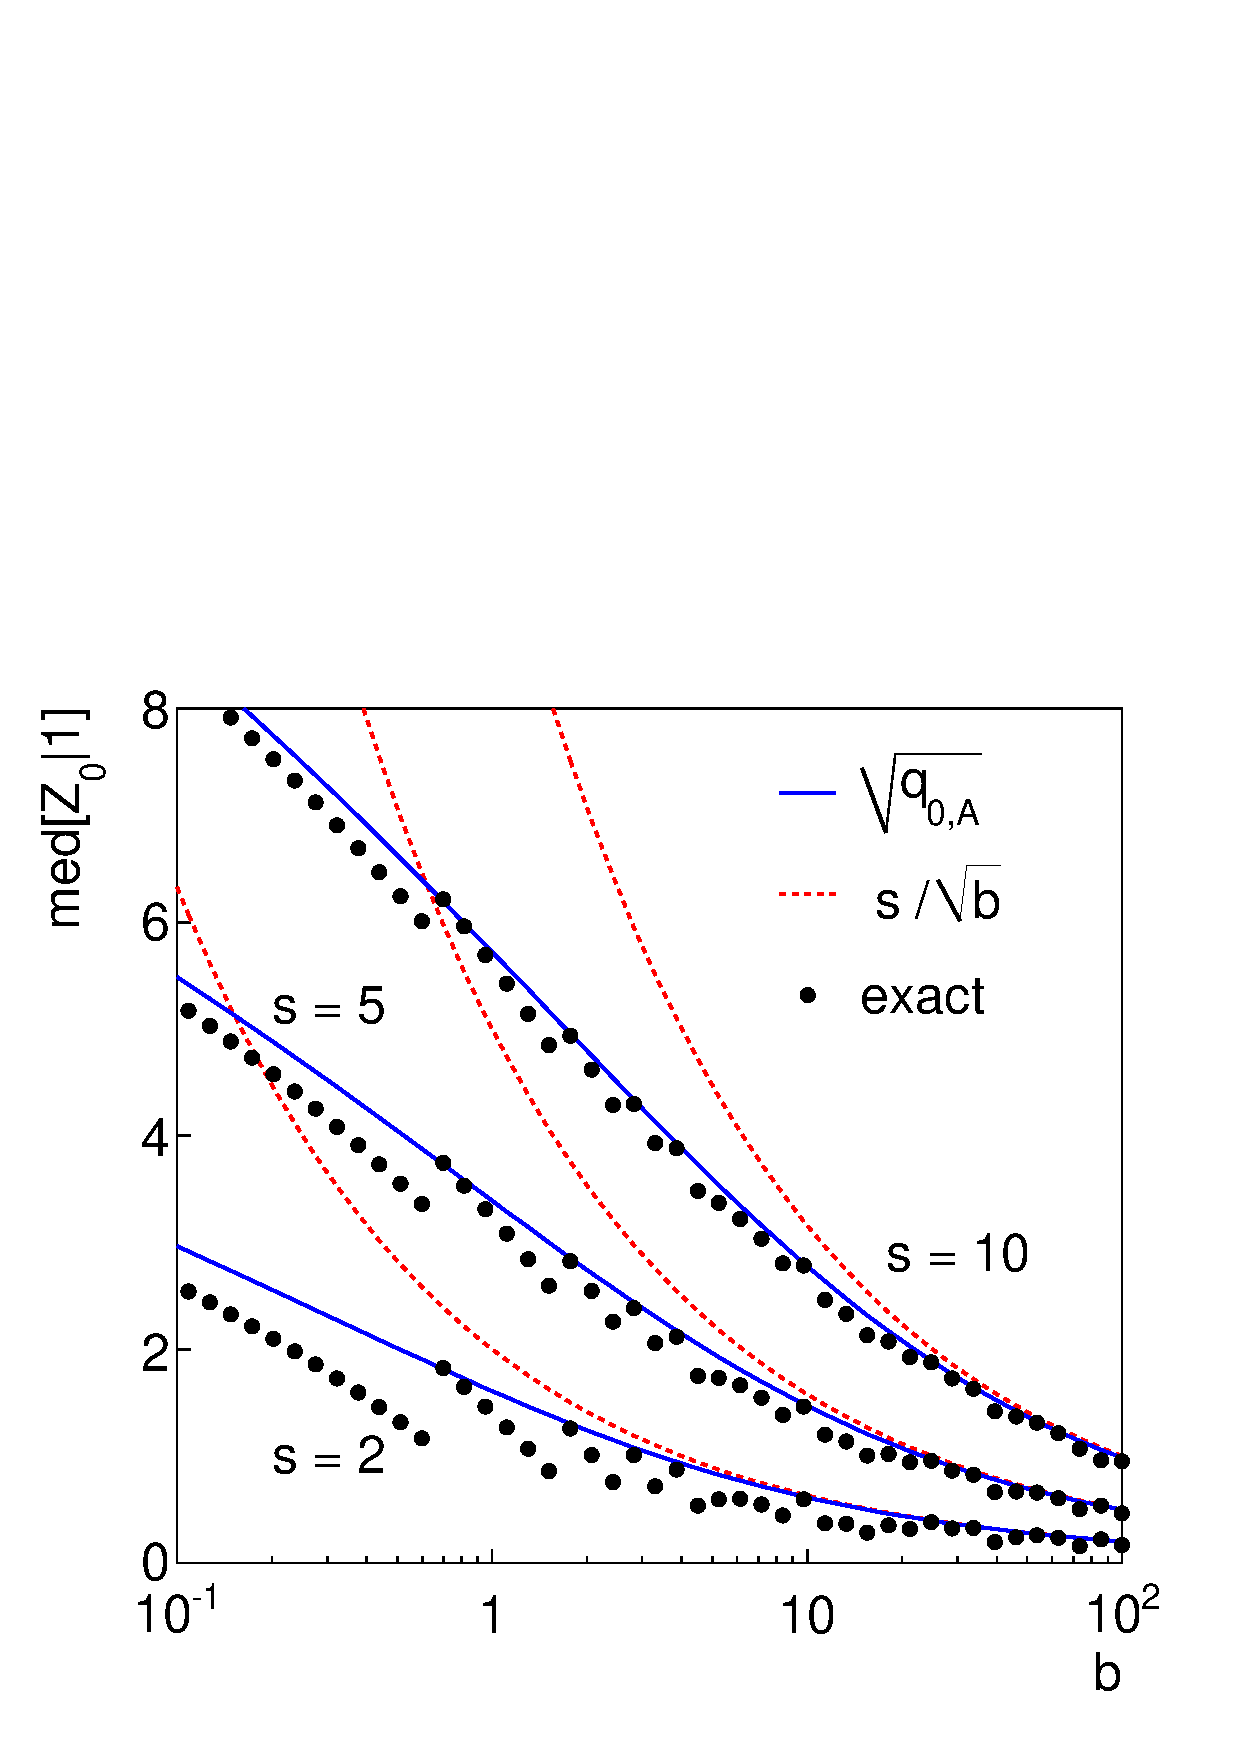
\includegraphics[width=\textwidth]{./medsig2.pdf}
  \end{minipage}\hfill
  \begin{minipage}[c]{0.45\textwidth}
    \caption{\small The median, assuming 
a mean number of signal events $s$, of the discovery significance $Z$ for different values of
$s$ and $b$ (from \cite{asimov,CowanPhystatAsimov}; see text).}
    \label{fig:medsig}
  \end{minipage}
  \hspace{0.05\textwidth}
\end{figure}
\renewcommand{\baselinestretch}{1}
\small\normalsize

\section{Poisson case with uncertain background}
\label{sec:bunknown}

If the expected number of background events, $b$, is not known one
must treat it as a nuisance parameter in the likelihood function.
Because $b$ could be adjusted to accommodate any observed number of
events, it would be impossible to reject the hypothesis of $s=0$
unless some additional information is introduced that constrains $b$.
Often this is done by means of a control measurement by counting the
number of events $m$ in a data sample where signal events are believed
to be absent, and where the mean number of events can be related to
the number of background events in the primary measurement of $n$.
For example, one may take $m$ as following a Poisson distribution with
a mean of $\tau b$, where $\tau$ is a scale factor that we take here
as known with negligible uncertainty.

The full likelihood function that describes both the primary measurement
$n$ and the control measurement $m$ is therefore the product of
the two corresponding Poisson distributions:

\begin{equation}
\label{eq:onoffL}
L(s,b) = \frac{(s+b)^n}{n!} e^{-(s+b)} \, 
\frac{(\tau b)^m}{m!} e^{-\tau b} \;.
\end{equation}

\noindent This problem has been studied in both particle physics and
astrophysics (see, e.g., \cite{asimov,LiMa83,Cranmer05,Cousins08}).
To find the profile likelihood ratio one needs the estimators for $b$
and $s$ as well as the conditional estimator for $b$ given a value of
$s$:

\begin{eqnarray}
\label{eq:shat}
\hat{s} & = & n - m/\tau \;, \\*[0.2 cm]
\label{eq:bhat}
\hat{b} & = & m/\tau \;, \\*[0.2 cm]
\label{eq:bhathat}
\hat{\hat{b}}(s) & = & \frac{ n + m - (1 + \tau) s + 
\sqrt{ (n + m - (1+\tau)s)^2 + 4 (1+\tau) s m } }{ 2 (1 + \tau) } \;.
\end{eqnarray}

\noindent For the statistic $q_0$ one needs in particular $\hat{\hat{b}}(0)$,
which from Eq.~(\ref{eq:bhathat}) is

\begin{equation}
\label{eq:bhathat0}
\hat{\hat{b}}(0) = \frac{n + m}{1 + \tau} \;.
\end{equation}

As in Sec.~\ref{sec:bknown} we use the approximation $Z = \sqrt{q_0}$, 
valid in the large sample limit, which gives

\begin{equation}
\label{eq:onoffZ}
Z = \left[ - 2 \left( 
n \ln \left[ \frac{ n + m }{ ( 1 + \tau) n } \right] +
m \ln \left[ \frac{ \tau (n + m)}{(1 + \tau) m } \right] \right) 
\right]^{1/2} \
\end{equation}

\noindent for $n > \hat{b}$ and $Z = 0$ otherwise.  This is the same
as Eq.~(17) of Ref.~\cite{LiMa83} and Eq.~(25) of
Ref.~\cite{Cousins08}.

As in Sec.~\ref{sec:bknown} we replace the data values $n$ and $m$
by their expectation values $s+b$ and $\tau b$ to give the
``Asimov'' approximation for the median significance.  Making
this substitution in Eq.~(\ref{eq:onoffZ}) gives

\begin{equation}
\label{eq:onoffmedZ}
Z_{\rm A} =  \left[ -2 \left( 
(s + b) \ln \left[ \frac{ s + (1+\tau)b}{(1+\tau)(s+b)} \right] +
\tau b \ln \left[ 1 + \frac{s}{(1+\tau)b} \right] \right) \right]^{1/2} \;.
\end{equation}

\noindent The case where the control measurement $m$ has a small
relative statistical uncertainty corresponds to $\tau$ very large, and
in this limit Eq.~(\ref{eq:onoffmedZ}) reverts to the expression for known
$b$ given by Eq.~(\ref{eq:Zmedcount}).

It is useful to re-express Eq.~(\ref{eq:onoffmedZ}) in terms of the
uncertainty one would quote on the background on the basis of the
control measurement $m$.  The estimator for $b$ is given by
Eq.~(\ref{eq:bhat}), and because the variance of $m$ is equal to its
mean, $\tau b$, the variance of $\hat{b}$ is

\begin{equation}
\label{eq:sigma2b}
V[\hat{b}] \equiv \sigma^2_b = \frac{b}{\tau} \;.
\end{equation}

\noindent Using this equation to eliminate $\tau$ from
(\ref{eq:onoffmedZ}) gives the result

\begin{equation}
\label{eq:onoffmedZ2}
Z_{\rm A} = \left[ 2 \left( (s+b)
\ln \left[ \frac{ (s+b)(b + \sigma_b^2) }{b^2 + (s+b) \sigma_b^2 } \right]
- \frac{b^2}{\sigma_b^2} \ln \left[ 1 +
\frac{ \sigma_b^2 s }{b (b + \sigma_b^2) } \right] \right) \right]^{1/2} \;.
\end{equation}

\noindent By expanding this expression in powers of $s/b$ and
$\sigma_b^2/b$ one finds

\begin{equation}
\label{eq:onoffmedZ3}
Z_{\rm A} = \frac{s}{\sqrt{b + \sigma_b^2}} \left( 1 + {\cal O}(s/b)
+ {\cal O}(\sigma_b^2/b) \right) \;.
\end{equation}

One sees that that the expression given in
Eq.~(\ref{eq:soverrootbsys}) and justified on intuitive grounds
results from the significance based on Wilks' theorem and use of the
Asimov data set.  The simple formula given by
Eq.~(\ref{eq:onoffmedZ3}) is expected to be valid in cases where one
has $s \ll b$ and $\sigma_b^2 \ll b$.  From Eq.~(\ref{eq:sigma2b}) we
have $\sigma_b^2/b = 1/\tau$, and because the expectation value of $m$
is $E[m] = \tau b$, the requirement $\sigma_b^2 \ll b$ is equivalent
to $E[m] \gg b$ or $\tau \gg 1$.  That is, the expected number of
events in the control region should be large compared to the expected
number of background events contributing to the primary measurement of
$n$ (and in addition $s \ll b$ must hold).

Figure~\ref{fig:medsigsys} shows the median discovery significance for
$s = 2, 5$ and $10$ as a function of $b$ for (left) several values of
$\sigma_b/b$ and (right) several values of $\tau$.  In each plot the
upper set of curves (points) corresponds to the smaller $\sigma_b/b$
or larger $\tau$.  The points are based on Eq.~(\ref{eq:onoffZ}) and
computed with Monte Carlo.  The structure in the points is due to the
discreteness of the Poisson distributed data.  The dashed and solid
curves show the predictions of Eqs.~(\ref{eq:soverrootbsys}) and
(\ref{eq:onoffmedZ2}), respectively.  Although both of these formulae
agree with the Monte Carlo values for sufficiently large $b$, the full
formula from Eq.~(\ref{eq:onoffmedZ2}) is clearly in far better
agreement for low $b$.  This is understandable because for decreasing
$b$ the ratios $s/b$ and $\sigma_b^2/b$ become large and thus the
approximation of Eq.~(\ref{eq:soverrootbsys}) is expected to break
down.

\setlength{\unitlength}{1.0 cm}
\renewcommand{\baselinestretch}{0.9}
\begin{figure}[h] \center
  %\vspace{-0.2 cm}
  %  \hspace{0.05\textwidth}
  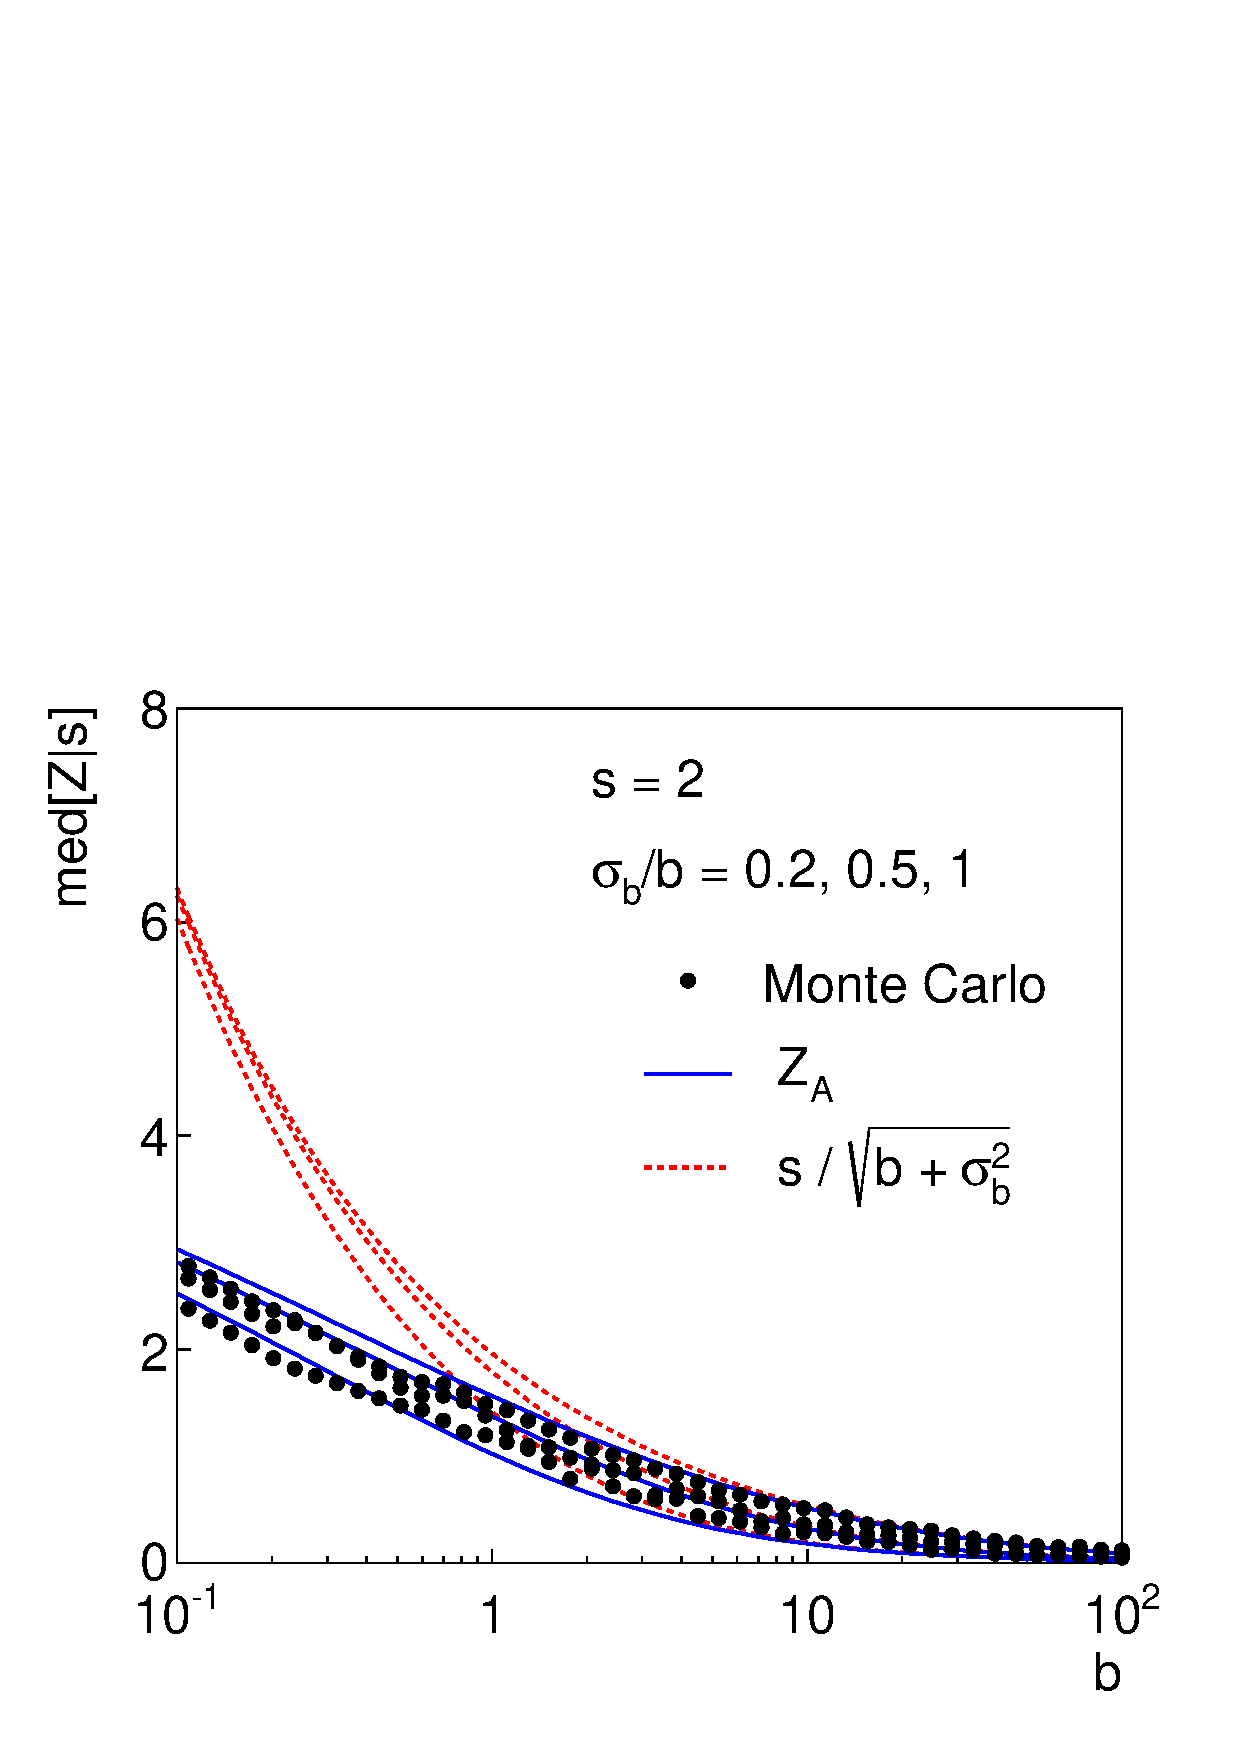
\includegraphics[width=0.35\textwidth]{./medsig_s2_rel.pdf}
  \hspace{0.1\textwidth}
    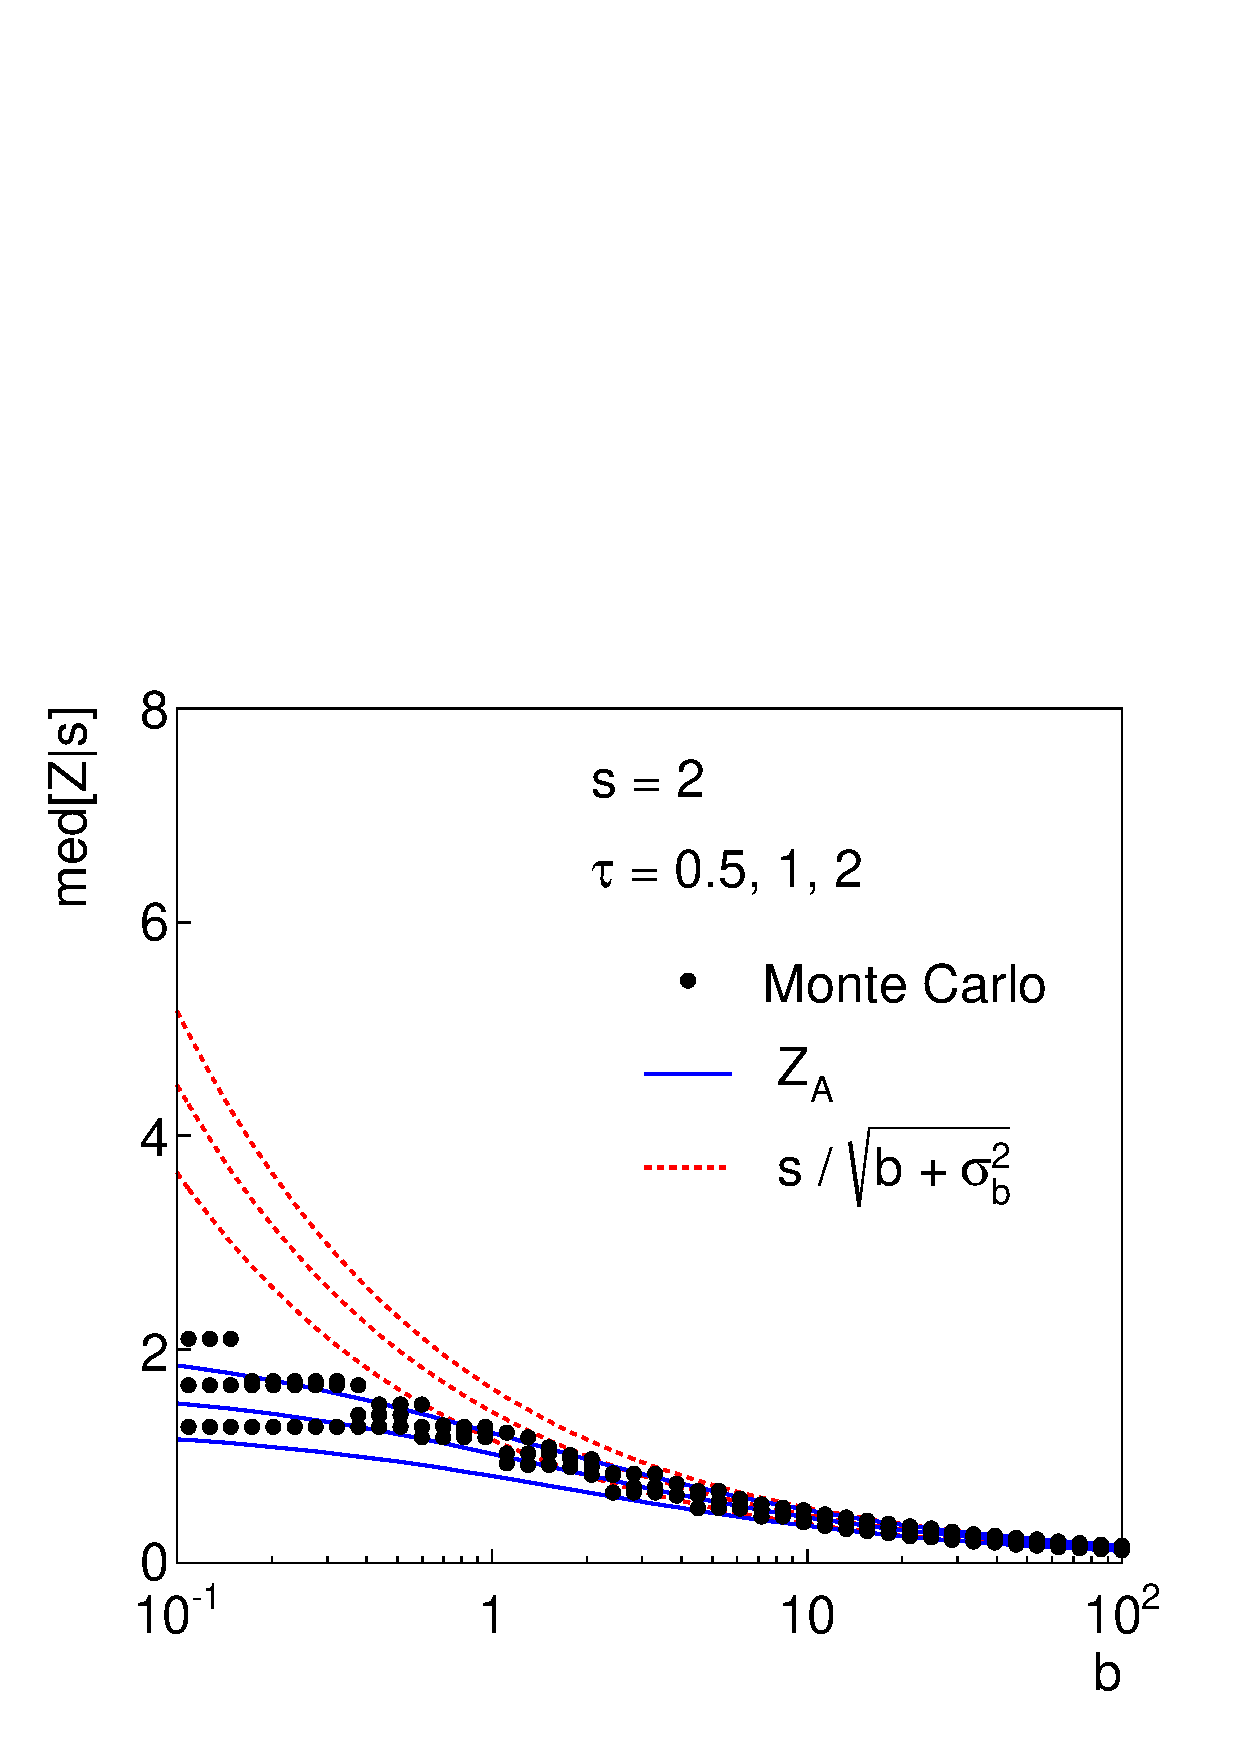
\includegraphics[width=0.35\textwidth]{./medsig_s2_tau.pdf}
\put(-14.0,3.5){(a)}
\put(1,3.5){(b)}
\vspace{0.2 cm}
  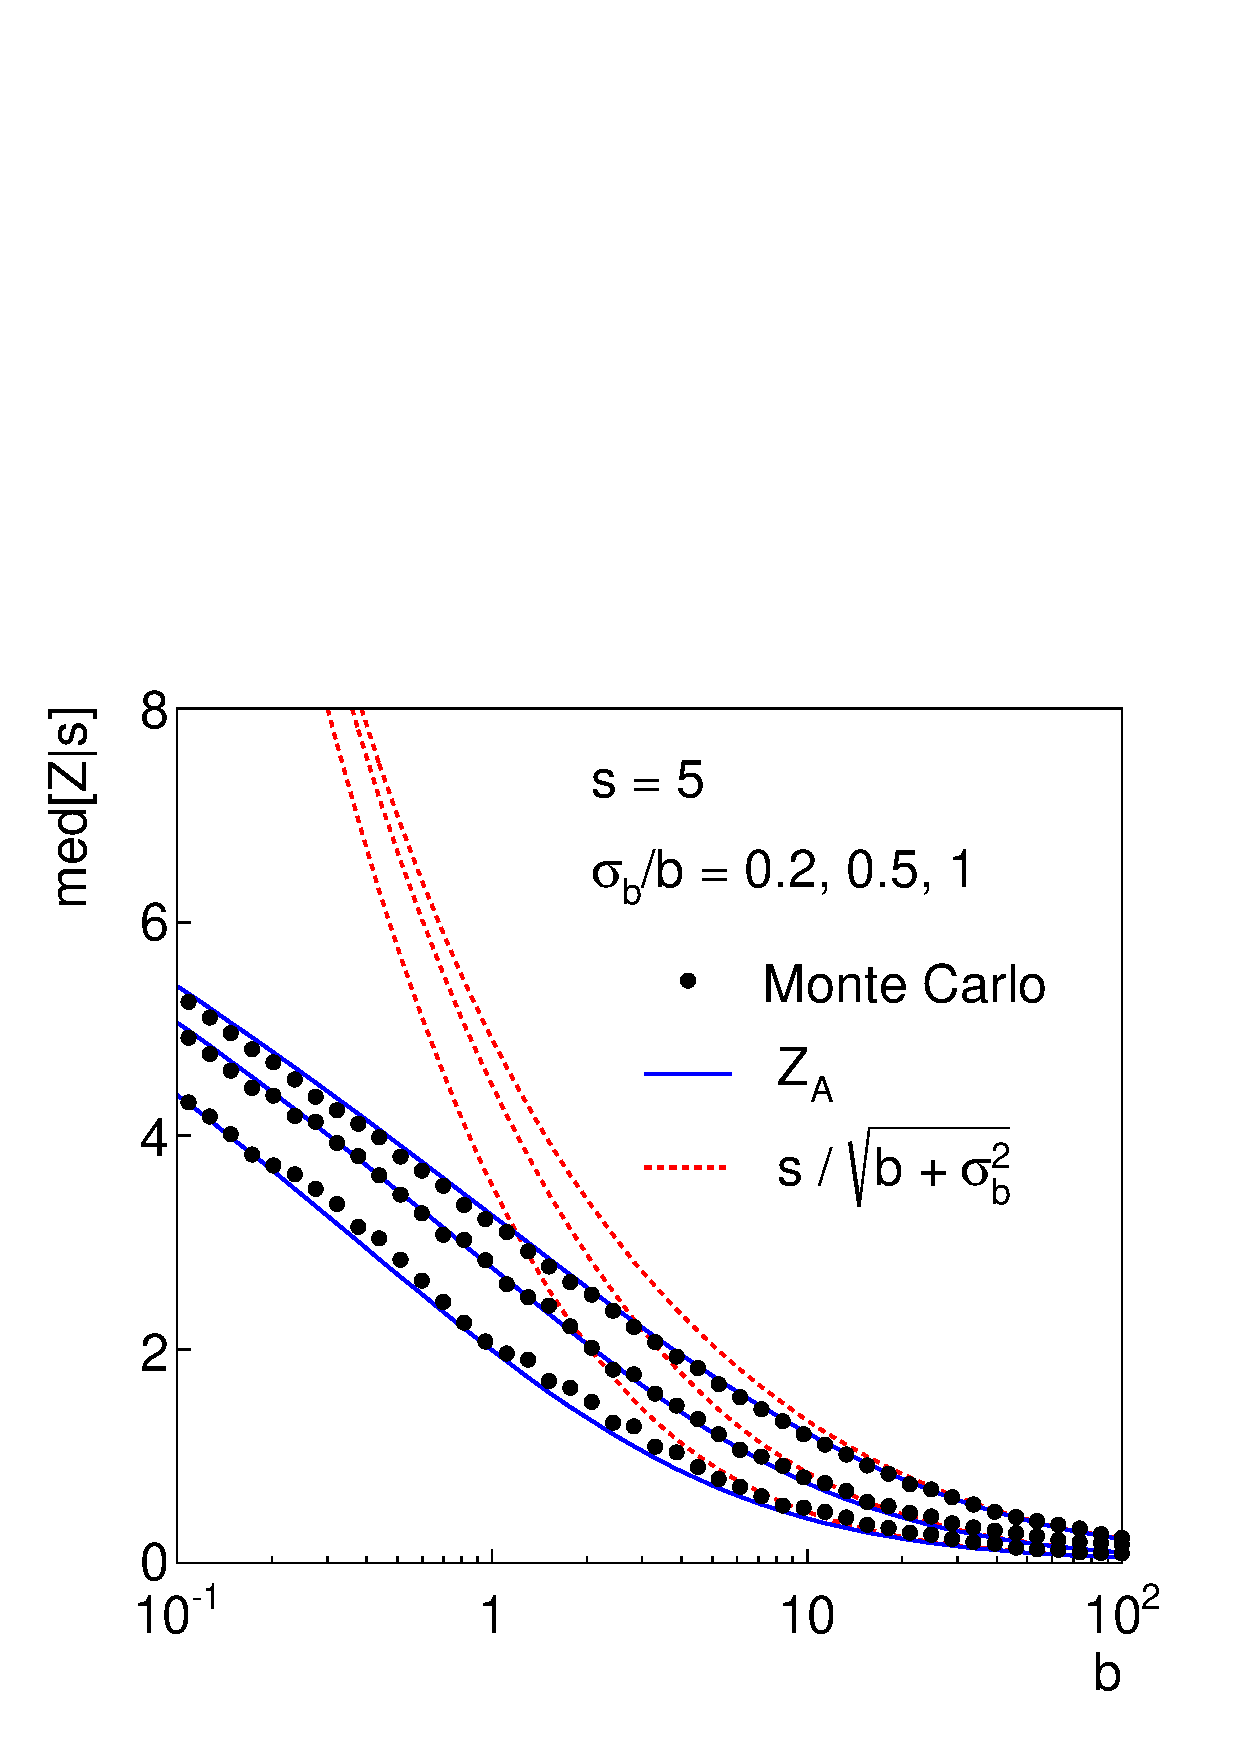
\includegraphics[width=0.35\textwidth]{./medsig_s5_rel.pdf}
  \hspace{0.1\textwidth}
    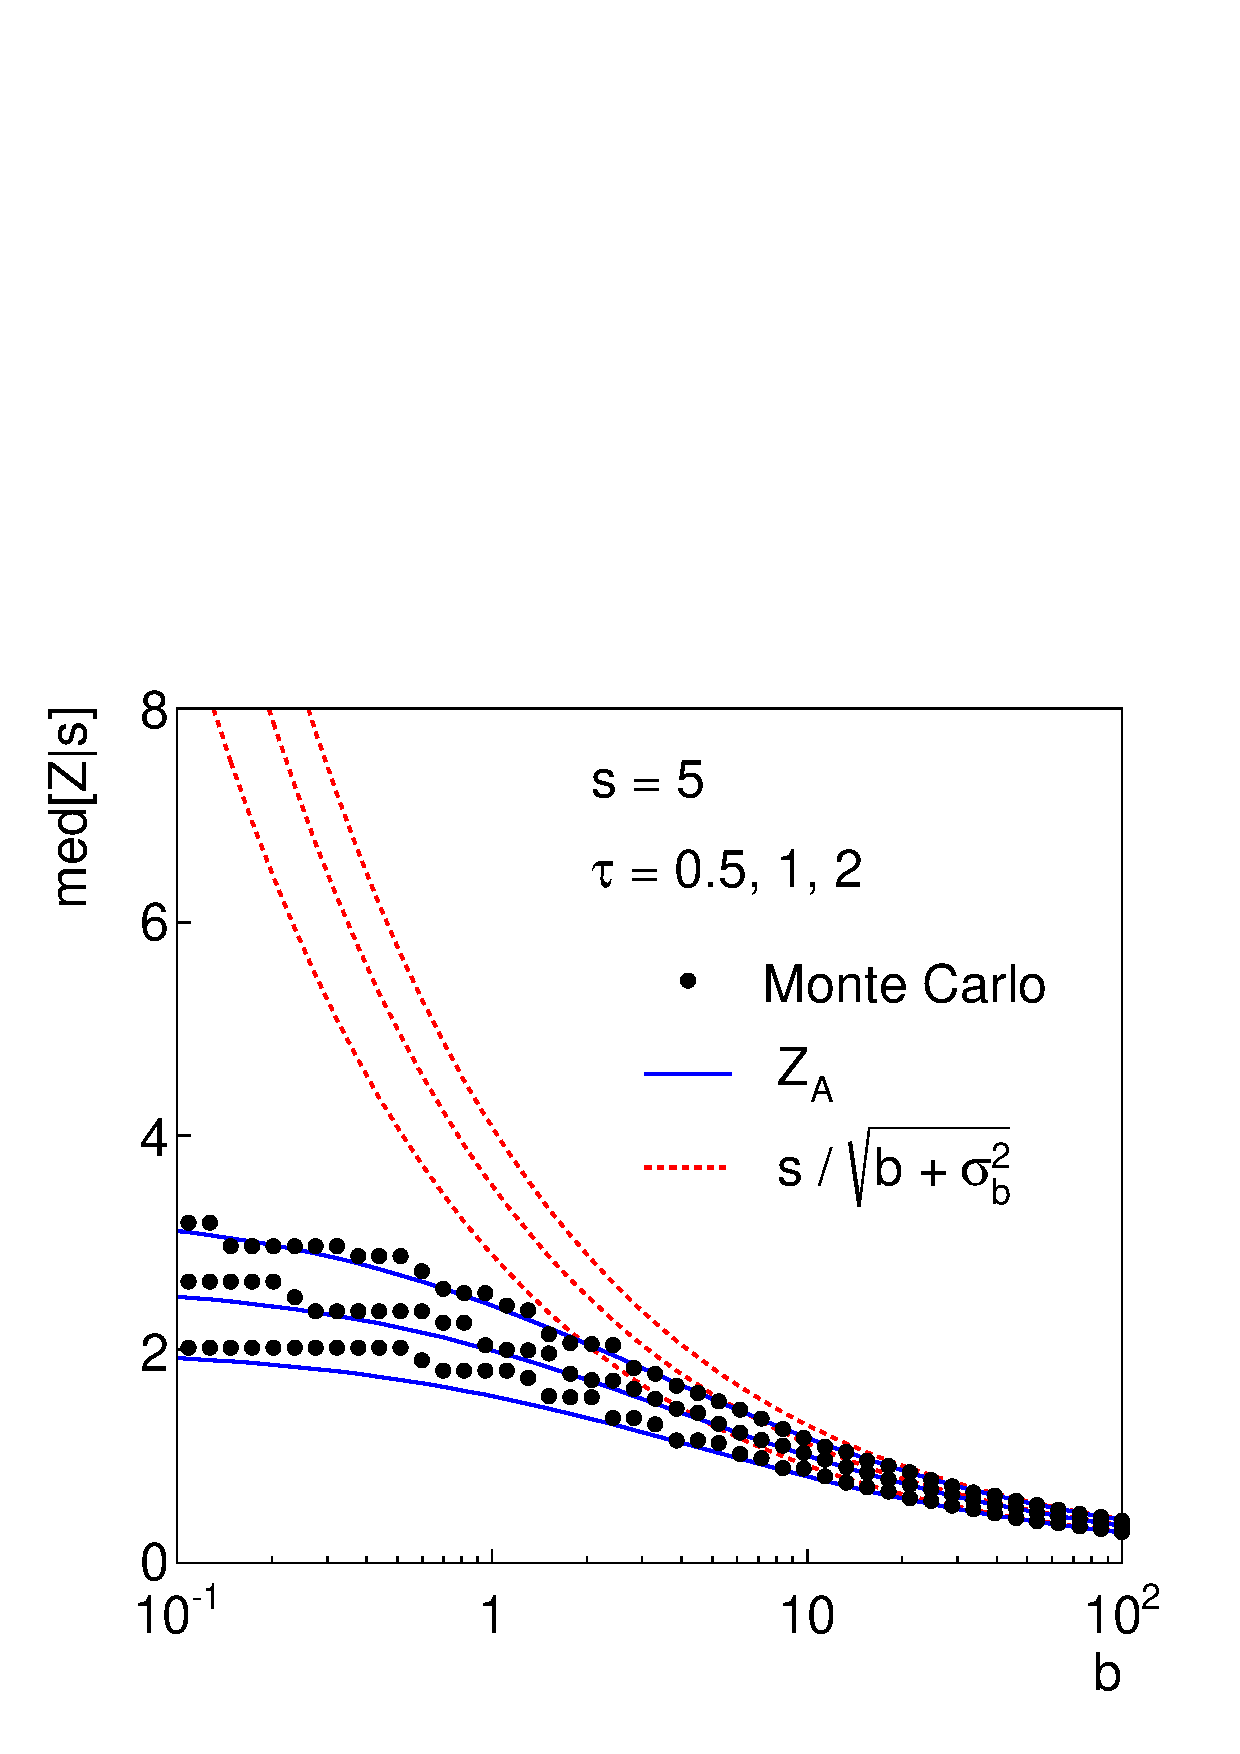
\includegraphics[width=0.35\textwidth]{./medsig_s5_tau.pdf}
\put(-14.0,3.5){(c)}
\put(1,3.5){(d)}
\vspace{0.2 cm}
  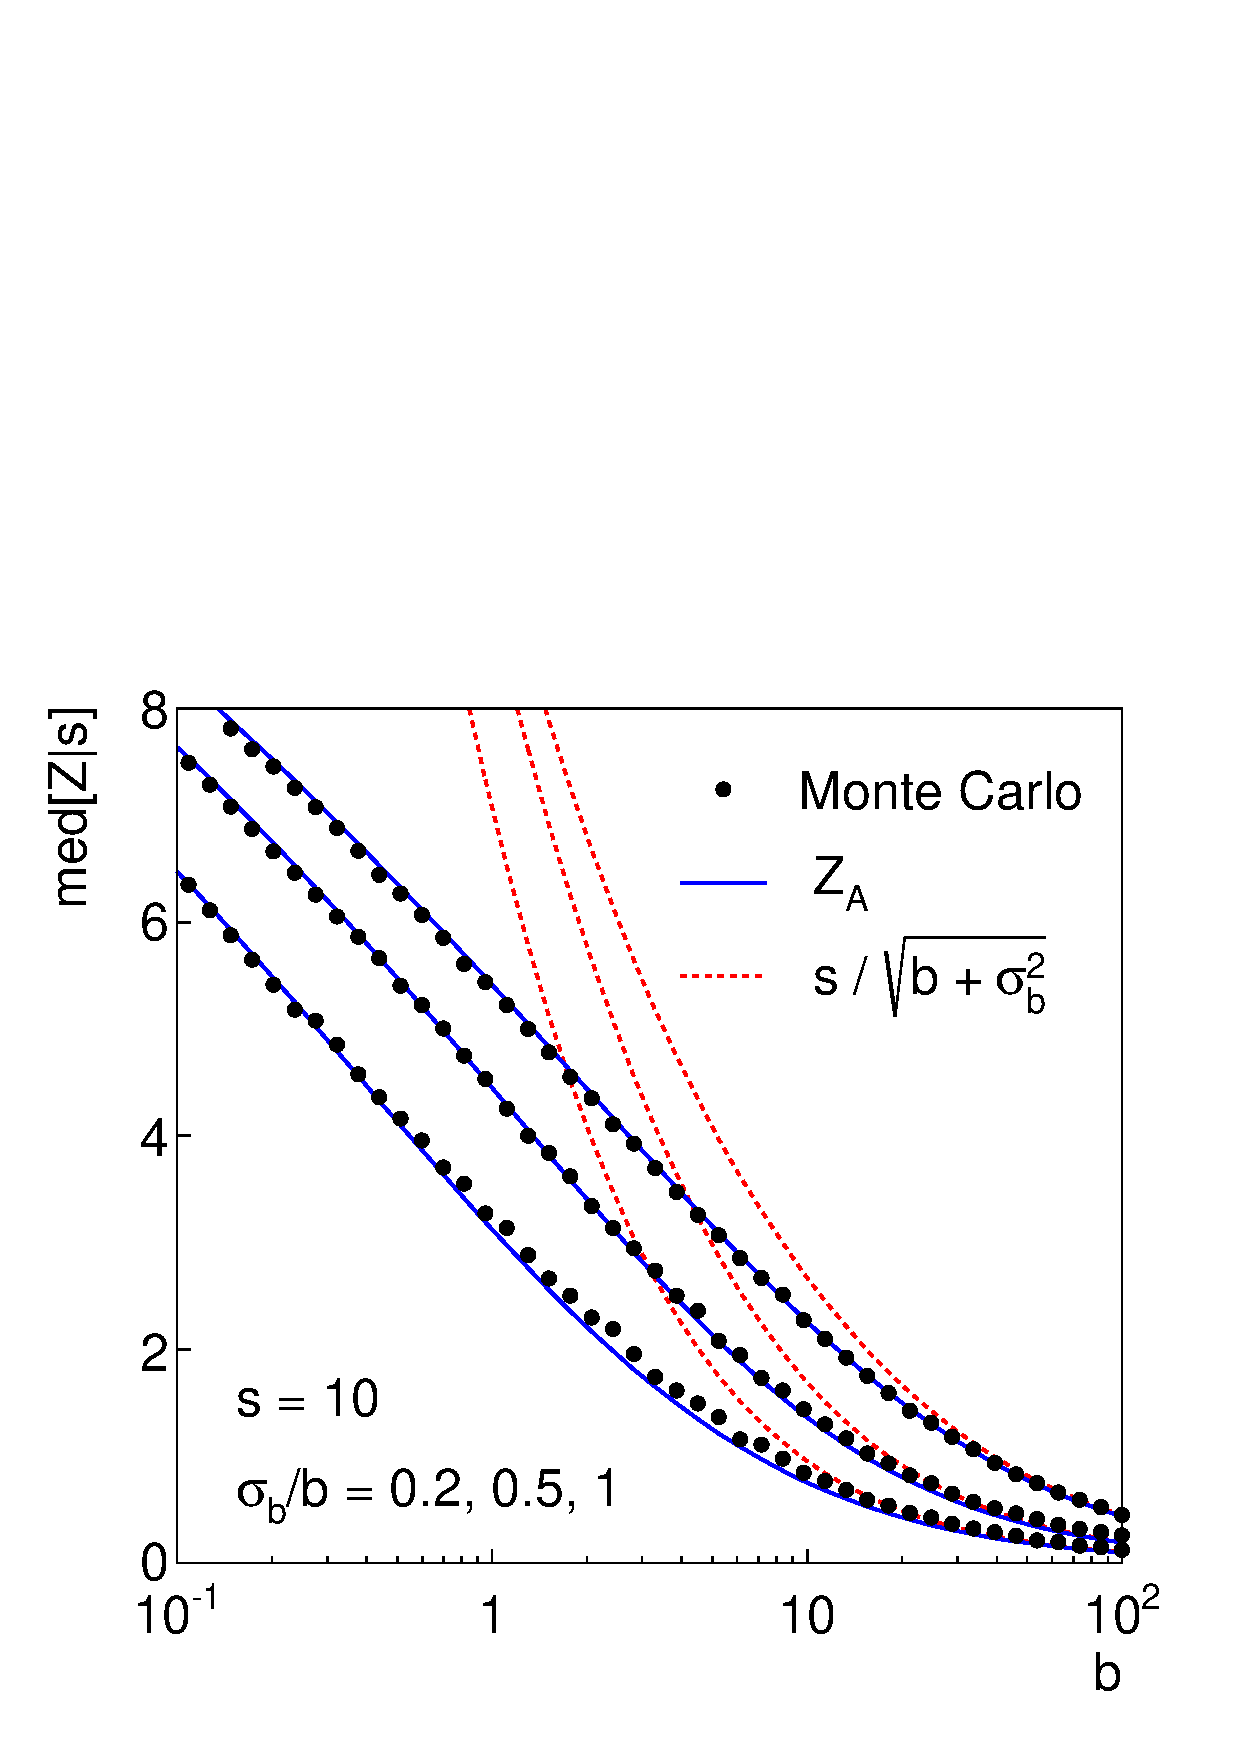
\includegraphics[width=0.35\textwidth]{./medsig_s10_rel.pdf}
  \hspace{0.1\textwidth}
    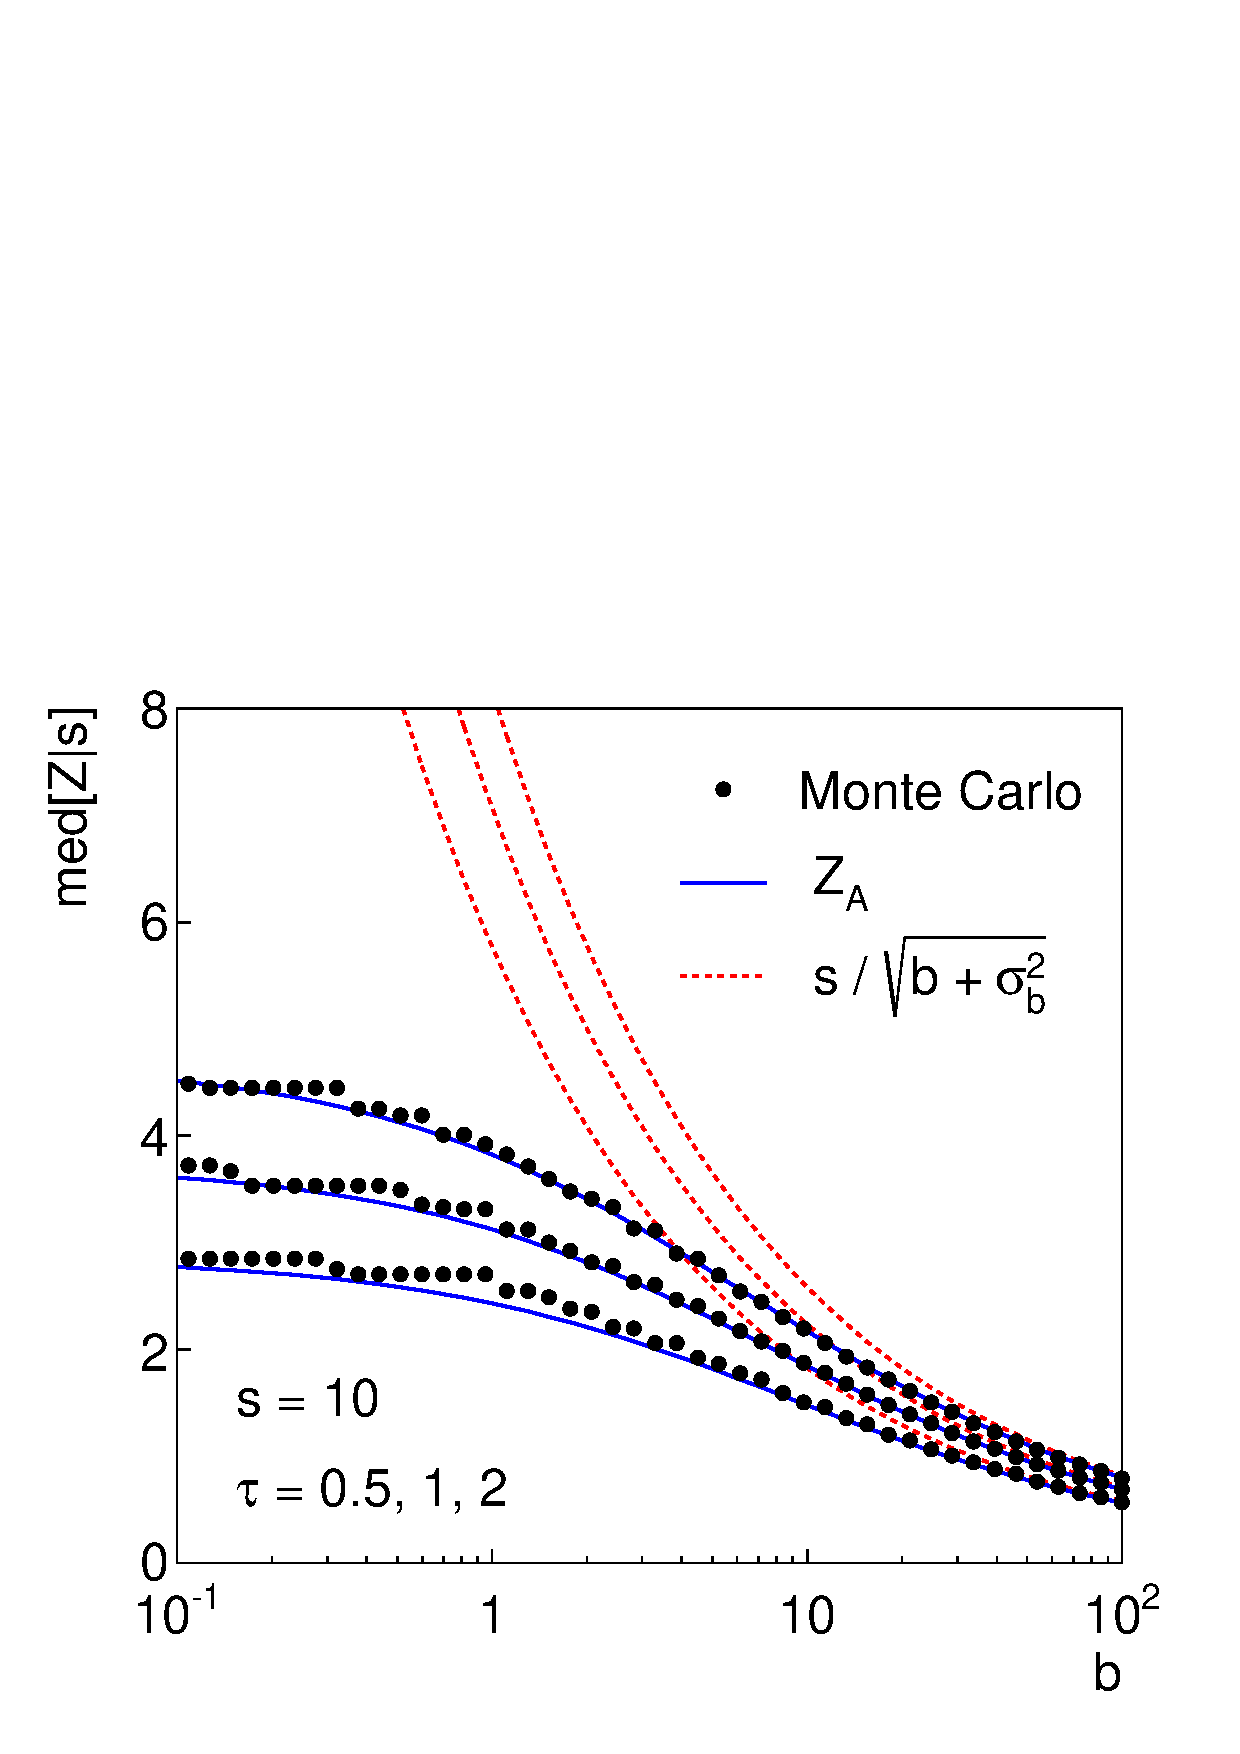
\includegraphics[width=0.35\textwidth]{./medsig_s10_tau.pdf}
\put(-14.0,3.5){(e)}
\put(1,3.5){(f)}
\vspace{0.2 cm}
\caption{\small The median, assuming 
an expected number of signal events $s = 2, 5$ and $10$
of the discovery significance $Z$ as a function of
the expected number of background events $b$ for 
(left) several values of $\sigma_b/b$ and (right) 
several values of $\tau$ (see text).}
    \label{fig:medsigsys}
    %  \hspace{0.05\textwidth}
      \vspace{-0.3 cm}
\end{figure}
\renewcommand{\baselinestretch}{1}
\small\normalsize

\section{Higher-order asymptotic corrections}
\label{sec:hoa}

Although the formulas shown above provide excellent approximations to the
expected significance for surprisingly small mean values of the Poisson-distributed number of events, one may still ask if even better accuracy 
can be achieved using higher-order corrections fo the asymptotic
distributions.


\section{Conclusions}
\label{sec:conclusions}

A simple expression for the expected discovery significance is given
by Eq.~(\ref{eq:onoffmedZ2}), which can be used for a counting
experiment in which the expected number of background events is
uncertain.  Specifically the formula treats the case where the
expected background is constrained by a control measurement consisting
of a Poisson distributed value.  In the limit of small background
uncertainty and also a small signal rate ($s \ll b$),
Eq.~(\ref{eq:onoffmedZ2}) reduces to Eq.~(\ref{eq:soverrootbsys}),
which has been used in particle physics.  The numerical studies shown,
however, indicate that for important ranges of background rate and
uncertainty, the limiting formula severely overestimates the expected
discovery significance, whereas the full formula is in very good
agreement with exact Monte Carlo results.


\begin{thebibliography}{[88]}
\bibitem{asimov} Glen Cowan, Kyle Cranmer, Eilam Gross and Ofer Vitells,
%{\it Asymptotic formulae for likelihood-based tests of new physics},
Eur.\ Phys.\ J.\ C 71 (2011) 1554.
\bibitem{CowanPhystatAsimov} Glen Cowan, {\it Use of the profile
likelihood function in searches for new physics} in 
H.~Prosper and L.~Lyons (eds.), 
Proceedings of the PHYSTAT 2011 Workshop, CERN-2011-006 (2011), p.~109.
Figure 1(a) in this paper corrects a minor numerical error in
Fig.~7 of Ref.~\cite{asimov}.
\bibitem{LiMa83} Tipei Li and Yuqian Ma, Astrophysical Journal 272
  (1983) 317--324.
\bibitem{Cranmer05}  Kyle Cranmer, {\it 
Statistical Challenges for Searches for New Physics at the LHC}, 
proceedings of PhyStat2005, Oxford; arXiv:physics/0511028.
\bibitem{Cousins08} Robert D.~Cousins, James T.~Linnemann and Jordan Tucker,
NIM A 595 (2008) 480--501; arXiv:physics/0702156.
%\bibitem{pdg} K. Nakamura et al. (Particle Data Group), J. Phys. G 37,
%  075021 (2010).
\end{thebibliography}

\end{document}
